% default values
\def\ttau{1} % Zeitkonstante tau

% Plot Umgebung:
\def\samples{41}

\def\xomegaordermin{-2}
\def\xomegaordermax{2}
\def\xomegamin{1e\xomegaordermin}
\def\xomegamax{1e\xomegaordermax}
\def\domain{\xomegamin:\xomegamax}

\def\yamptiefmin{0.6e-2}    % \ymin needed as macro to draw ycomb with node-text from x-axis to plot
\def\yamptiefmax{2}

\def\yamphochmin{0.6e-2}    % \ymin needed as macro to draw ycomb with node-text from x-axis to plot
\def\yamphochmax{2}

\def\yphitiefmax{+10}
\def\yphitiefmin{-100}      % \ymin needed as macro to draw ycomb with node-text from x-axis to plot % 1. Ordnung
\def\yphitiefg{-45}

\def\yphihochmin{-10}       % \ymin needed as macro to draw ycomb with node-text from x-axis to plot % 1. Ordnung % Alternative: [ycomb, update limits=false] small y value outer bounds but no dynamic node text
\def\yphihochmax{100}
\def\yphihochg{45}

%%%%%%%%%%%%%%%%%%%%%%%%%%%%%%%%%%%%%%%%%%%%%%%%%%%%%%%%%%%%%%%%%%%%%%%%%%%%

% RC-Tiefpass 1. Ord. Phasengang
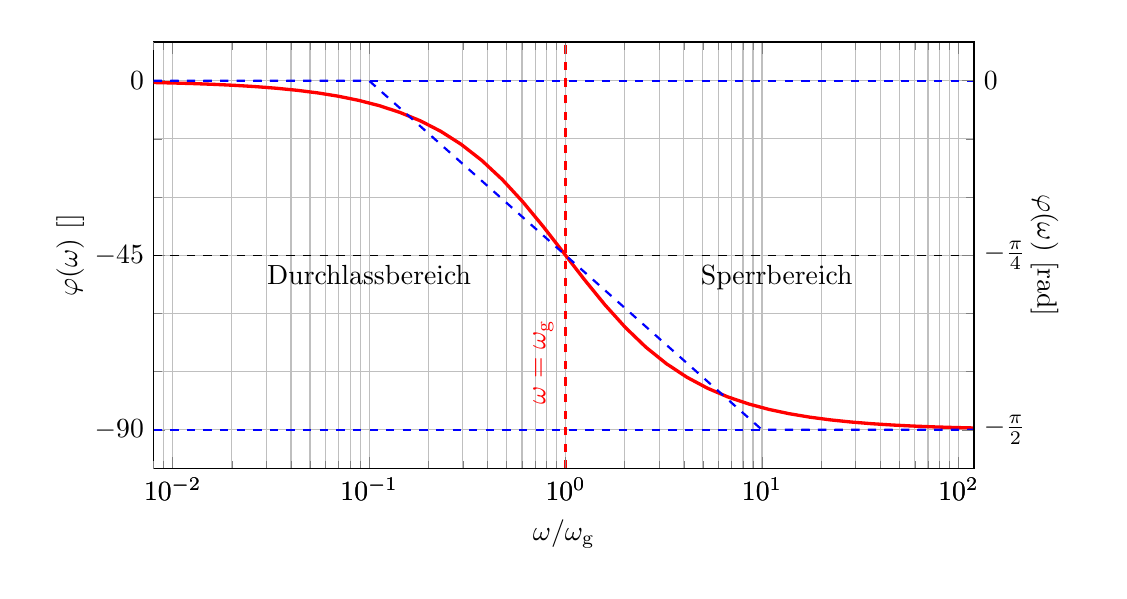
\begin{tikzpicture}[x=1mm,y=1mm] % gilt für tikz-coordinaten außerhalb der axis-environment
    \draw[draw=none] (-16,-13) rectangle (120,56); % Bildrahmen, Koordinatenbezug auf (0,0) des \begin{axis}...\end{axis} pgfplots, für
    \begin{axis}[
        %title={Phasengang RC-Tiefpass 1. Ordnung},
        xmode=log,ymode=normal,
        xlabel={$\omega/\omega_{\mathrm{g}}$},
        ylabel={$\varphi(\omega)\ [\degree]$},
        ylabel shift = -3 pt,
        xmin=0.8*\xomegamin, xmax=1.2*\xomegamax,
        ymin=\yphitiefmin, ymax=\yphitiefmax,
        minor y tick num= 2,
        domain=0.8*\xomegamin:1.2*\xomegamax,
        samples=\samples,
        width=12cm,
        height=7cm,
        ytick={0,-45,-90},
        yticklabels={$0$,$-45$,$-90$},
        grid=both,
        mark=none,
    ]     
        % Beschriftung
        \addplot[draw=none,black]  coordinates { (\xomegamin, -45) ( 1.000, -45) } node[pos=0.5,below]{Durchlassbereich}; % Bereich
        \addplot[draw=none,black]  coordinates { (1.414, -45) ( \xomegamax, -45) } node[pos=0.5,below]{Sperrbereich};    % Bereich

        % Plot
        \addplot[very thick,red,]   {atan(-\x*\ttau)};

        % Näherung, Hilfslinien
        \addplot[dashed,black,]     coordinates { (0.8*\xomegamin, -45) (1.2*\xomegamax, -45) };% -45deg
        \addplot[dashed,blue,thick] coordinates { (0.8*\xomegamin, -90) (1.2*\xomegamax, -90) };% -90deg, Asymptote
        \addplot[dashed,blue,thick] coordinates { (0.8*\xomegamin, +00) (1.2*\xomegamax, +00) };% +00deg, Asymptote
        \addplot[dashed,blue,thick] coordinates { (0.8*\xomegamin, +00) (0.1,0) (10,-90) (1.2*\xomegamax, -90) }; % Näherung, Gerade
        \addplot[dashed,red,thick,] coordinates { (1/(\ttau),\yphitiefmin) (1/(\ttau),\yphitiefmax) }% omega=omega_g
            node [pos=0.25,sloped,style={yshift=8pt}] {$\omega=\omega_{\mathrm{g}}$};                

    \end{axis}
    \begin{axis}[
        xmode=log,ymode=normal,
        axis y line*=right, 
        ylabel={$\varphi(\omega)\ [\mathrm{rad}]$},
        ylabel shift = -5 pt,
        ylabel style={rotate=180},
        xmin=0.8*\xomegamin, xmax=1.2*\xomegamax,
        ymin=\yphitiefmin, ymax=\yphitiefmax,
        minor y tick num= 2,
        width=12cm,
        height=7cm,
        ytick={0,-45,-90},
        yticklabels={$0$,$-\frac{\pi}{4}$,$-\frac{\pi}{2}$},
        grid=none,
    ]
    \end{axis}
\end{tikzpicture}%